\documentclass[conference]{IEEEtran}
\IEEEoverridecommandlockouts
\usepackage{cite}
\usepackage{amsmath,amssymb,amsfonts}
\usepackage{graphicx}
\usepackage{booktabs}
\usepackage{siunitx}
\usepackage{xcolor}
\usepackage{tikz}
\usetikzlibrary{arrows.meta,positioning,fit,backgrounds,calc}
\usepackage[hidelinks]{hyperref}
\sisetup{detect-all,group-separator={,},group-minimum-digits=4}
\graphicspath{{figures/}}
\def\repourl{https://github.com/Sean-KSH/silicon-atlas}
\def\demourl{https://sean-ksh.github.io/silicon-atlas/}

\begin{document}

\title{Silicon Atlas: An Interactive, Verified Platform for\\Teaching Semiconductor Materials and Devices}

\author{\IEEEauthorblockN{Sean Kim}
\IEEEauthorblockA{Department of Electrical and Computer Engineering\\
Princeton University, Princeton, NJ 08544, USA}}

\maketitle

\begin{abstract}
Introductory courses on solid-state and electronic/photonic devices ask students to connect a chain of ideas: how a wafer is made, how bands and carriers arise, how carriers move, and how junctions, transistors, and optical devices behave and are measured. Textbooks present these as separate chapters, and the models behind them are rarely something a student can change and watch respond. This paper presents Silicon Atlas, an open-source set of ten interactive labs that runs in a web browser and follows that chain from silica to a measurement bench. Each lab is driven by a small, documented physics kernel: Scheil segregation, quantum wells and tunneling, Fermi--Dirac charge neutrality, a finite-volume continuity solver, Deal--Grove oxidation and dopant diffusion, depletion and Poisson--Boltzmann junction electrostatics, the Shockley diode, the MOS capacitor and long-channel MOSFET, photodiodes and solar cells, and transistor-level circuit measurements. All kernels share one set of material parameters, state their assumptions, and refuse inputs outside their supported range. Every kernel is verified against reference results recomputed independently in Python. Closed-form results agree to within $10^{-14}$ in relative terms, the Fermi--Dirac integral to $1.1\times10^{-8}$, and the remaining numerical schemes converge at their expected rates, with the first-order cases identified. The labs add learning goals, guided predictions, and self-check questions, and are intended for class demonstrations and independent study. No comparison with measured data or study of learning outcomes has yet been made.
\end{abstract}

\begin{IEEEkeywords}
Semiconductor devices, engineering education, interactive simulation, p--n junction, MOSFET, Poisson--Boltzmann, verification.
\end{IEEEkeywords}

%======================================================================
\section{Introduction}
%======================================================================
A first course on semiconductor devices builds a long argument. Purified, single-crystal silicon has energy bands; doping sets the carrier populations; carriers drift and diffuse; a p--n junction forms a field that controls injection; a gate controls a channel; light creates carriers that a junction collects; and a measurement bench reveals all of this through currents and voltages. Standard texts develop each step carefully \cite{neamen2012,sze2007}, but a student meets them as separate chapters, each with its own figures, and rarely gets to ask what happens to a later step when an earlier one changes.

Interactive simulations can help with that question when they respond to a change in a way that is physically consistent and explained. Silicon Atlas is built around that idea. It is a set of ten browser-based labs that follow one path through an introductory course, from silica to a measurement bench (Fig.~\ref{fig:map}). In each lab the student changes one input, such as a doping level, a bias, a wavelength, or a process step, and every linked diagram and plot updates from the same calculation. A panel then states in words what changed and which quantities were held fixed.

Two goals shaped the design. The first was that every result shown should come from a model that is simple enough to explain in class, with its assumptions stated and its range enforced. The second was that the code should be checked the way a numerical paper is checked: each physics kernel is compared with reference results computed independently, and the agreement is reported. The platform is meant to support teaching, not to predict device or process behavior, and this paper reports verification of the implementation rather than validation against measurements.

The contributions are as follows.
\begin{enumerate}
\item Ten connected labs covering crystal growth, quantum and band foundations, equilibrium statistics, transport, a four-mask metal-gate nMOS process, junction electrostatics, diode current, MOS devices, photonic devices, and transistor-level measurements, with a shared course guide, learning goals, guided predictions, and self-check questions (Section~\ref{sec:design}).
\item An architecture in which every physics kernel is independent of the interface, uses SI units, draws on one shared parameter set, and withholds results outside its supported range (Section~\ref{sec:arch}).
\item A compact statement of each model and numerical method, including the choices made where textbook sources disagree (Section~\ref{sec:models}).
\item A verification suite that recomputes each result with NumPy and SciPy and reports the error and convergence order, together with 89 automated test groups that run on every change (Section~\ref{sec:verification}).
\end{enumerate}

\begin{figure*}[t]
\centering
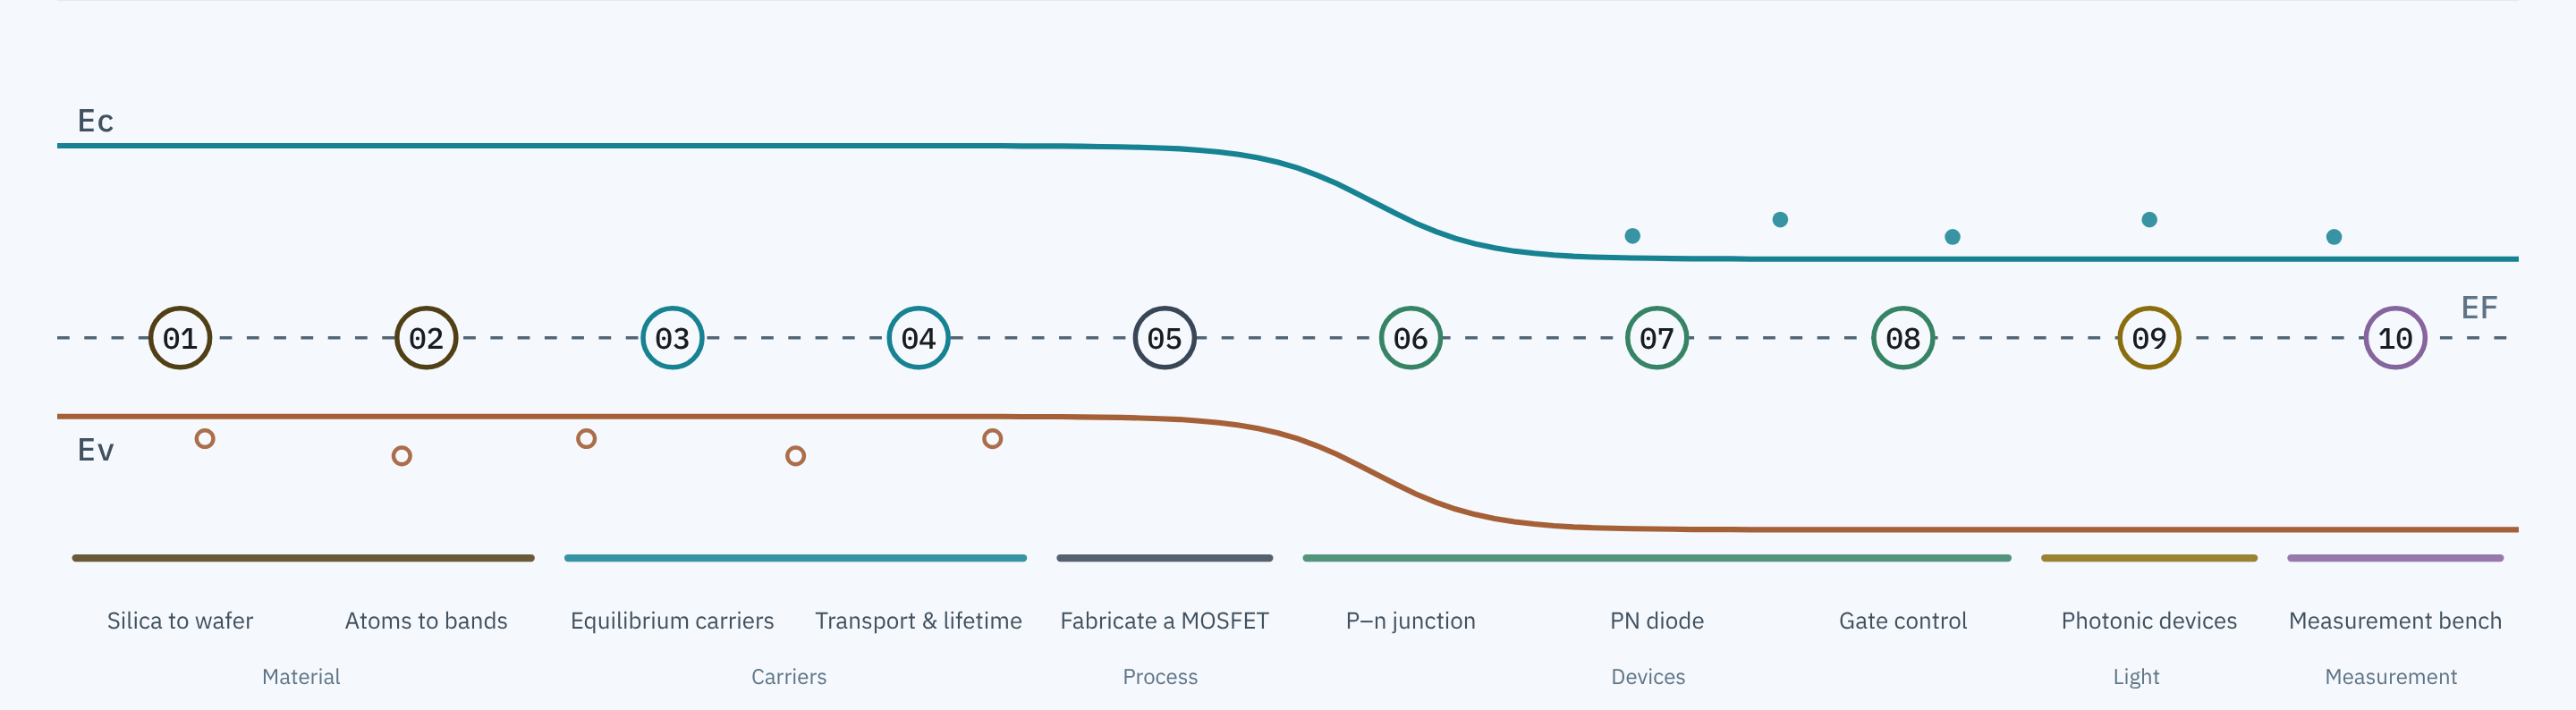
\includegraphics[width=\textwidth]{fig_map.png}
\caption{Course guide of Silicon Atlas. The ten labs are drawn on the Fermi level of a stylized p--n junction band diagram, grouped by stage (material, carriers, process, devices, light, measurement). The bands step down at module~06, the p--n junction. The drawing is a map, not a calculated band diagram.}
\label{fig:map}
\end{figure*}

%======================================================================
\section{Related Work}
%======================================================================
PhET simulations showed that carefully designed interactive simulations can support conceptual learning in introductory physics, and set a standard for interfaces that invite exploration while hiding unnecessary complexity \cite{wieman2008}. In semiconductor devices, nanoHUB hosts many simulation tools for education and research, several of which solve drift--diffusion or Schr\"odinger--Poisson problems with research-grade numerical methods \cite{klimeck2008}. Commercial TCAD tools go further, coupling process and device simulation on two- and three-dimensional meshes using methods such as the Scharfetter--Gummel discretization \cite{scharfetter1969,selberherr1984}.

Silicon Atlas sits between these. Its models are the ones introduced in an undergraduate text \cite{neamen2012}, in one dimension or as lumped elements, so a student can follow every equation from the panel to the plot. Unlike a collection of separate tools, the labs share one parameter set and one interface, and one lab's output can be passed to another: the fabricated device in the process lab can be imported into the MOS lab. The guided experiments follow a predict--observe--explain pattern \cite{white1992}, in line with evidence that active engagement improves learning in STEM courses \cite{freeman2014}. Any such benefit for this platform remains to be measured.

%======================================================================
\section{Educational Design}\label{sec:design}
%======================================================================
\subsection{Modules and course paths}
Table~\ref{tab:modules} lists the ten labs, their models, and the matching textbook chapters. A lab can be used on its own, and each one lists the labs it builds on. The course guide suggests two orders. A solid-state device physics path follows the order of a physics text (modules 02, 03, 04, 06, 07, 08, 09; about 3~h). An electronic and photonic devices path starts from fabrication and ends at the measurement bench (01, 05, 03, 06, 07, 08, 09, 10; about 3.5~h).

\begin{table}[t]
\centering
\caption{The ten labs, their main models, and textbook chapters \cite{neamen2012}}
\label{tab:modules}
\scriptsize
\setlength{\tabcolsep}{2.5pt}
\begin{tabular}{@{}r p{19mm} p{38mm} l@{}}
\toprule
\# & Lab & Main model & Ch. \\
\midrule
01 & Silica to wafer & Scheil segregation; interface heat balance & 1 \\
02 & Atoms to bands & Infinite well; rectangular barrier; 1D tight binding & 1--3 \\
03 & Equilibrium carriers & Charge neutrality, Boltzmann or Fermi--Dirac & 4 \\
04 & Transport \& lifetime & 1D continuity equation, finite volume & 5--6 \\
05 & Fabricate a MOSFET & Deal--Grove; dopant diffusion; resist threshold & -- \\
06 & P--n junction & Depletion; equilibrium Poisson--Boltzmann & 7 \\
07 & PN diode & Shockley diode, finite neutral regions; charge control & 8 \\
08 & Gate control & MOS first integral; gradual-channel MOSFET & 10--11 \\
09 & Photonic devices & Beer--Lambert generation; illuminated diode & 14 \\
10 & Measurement bench & Square-law circuits; instrument error models & 11 \\
\bottomrule
\end{tabular}
\end{table}

\subsection{Structure of a lab}
Every lab follows the same sequence, so a student learns the interface once. It opens with three learning goals, a time estimate, the reading, and its prerequisites. A set of controls and presets drives several linked views, for example six spatially aligned plots of doping, carriers, charge, field, potential, and band energies in the junction lab (Fig.~\ref{fig:ui}). A panel titled ``What changed and why?'' explains the response and names the quantities held fixed. Guided experiments ask the student to write a prediction before applying a preset and revealing the explanation. Expandable panels give the equations, assumptions, and sources, and a ``Deeper physics'' view adds detail for students who want it. Each lab ends with two self-check questions whose answers are hidden until requested.

\subsection{Honesty in the interface}
Three rules apply throughout. First, calculated results are kept separate from illustrations: schematic equipment, animated carriers, and the one-orbital band model are labeled as illustrations, and exaggerated vertical scales are labeled. Second, equilibrium and biased conditions are kept separate: the Poisson--Boltzmann solver runs only at zero bias, and the equilibrium Fermi level is removed from band diagrams under bias. Third, when an input leaves the range where a model holds, for example beyond low injection, above a conservative field limit, or below the long-channel length, the lab reports the reason and withholds the result instead of drawing it.

\subsection{Classroom tools}
For instructors, the course guide gives a ten-minute demonstration for each lab, built from presets that restore tested settings. A presenting mode enlarges the page for projectors, a light theme suits lit rooms and printing, a ``Copy link'' button encodes the current settings in the URL so a slide or assignment can open an exact setup, and printing a lab produces a handout with its goals and self-check questions but not the answers.

\begin{figure*}[t]
\centering
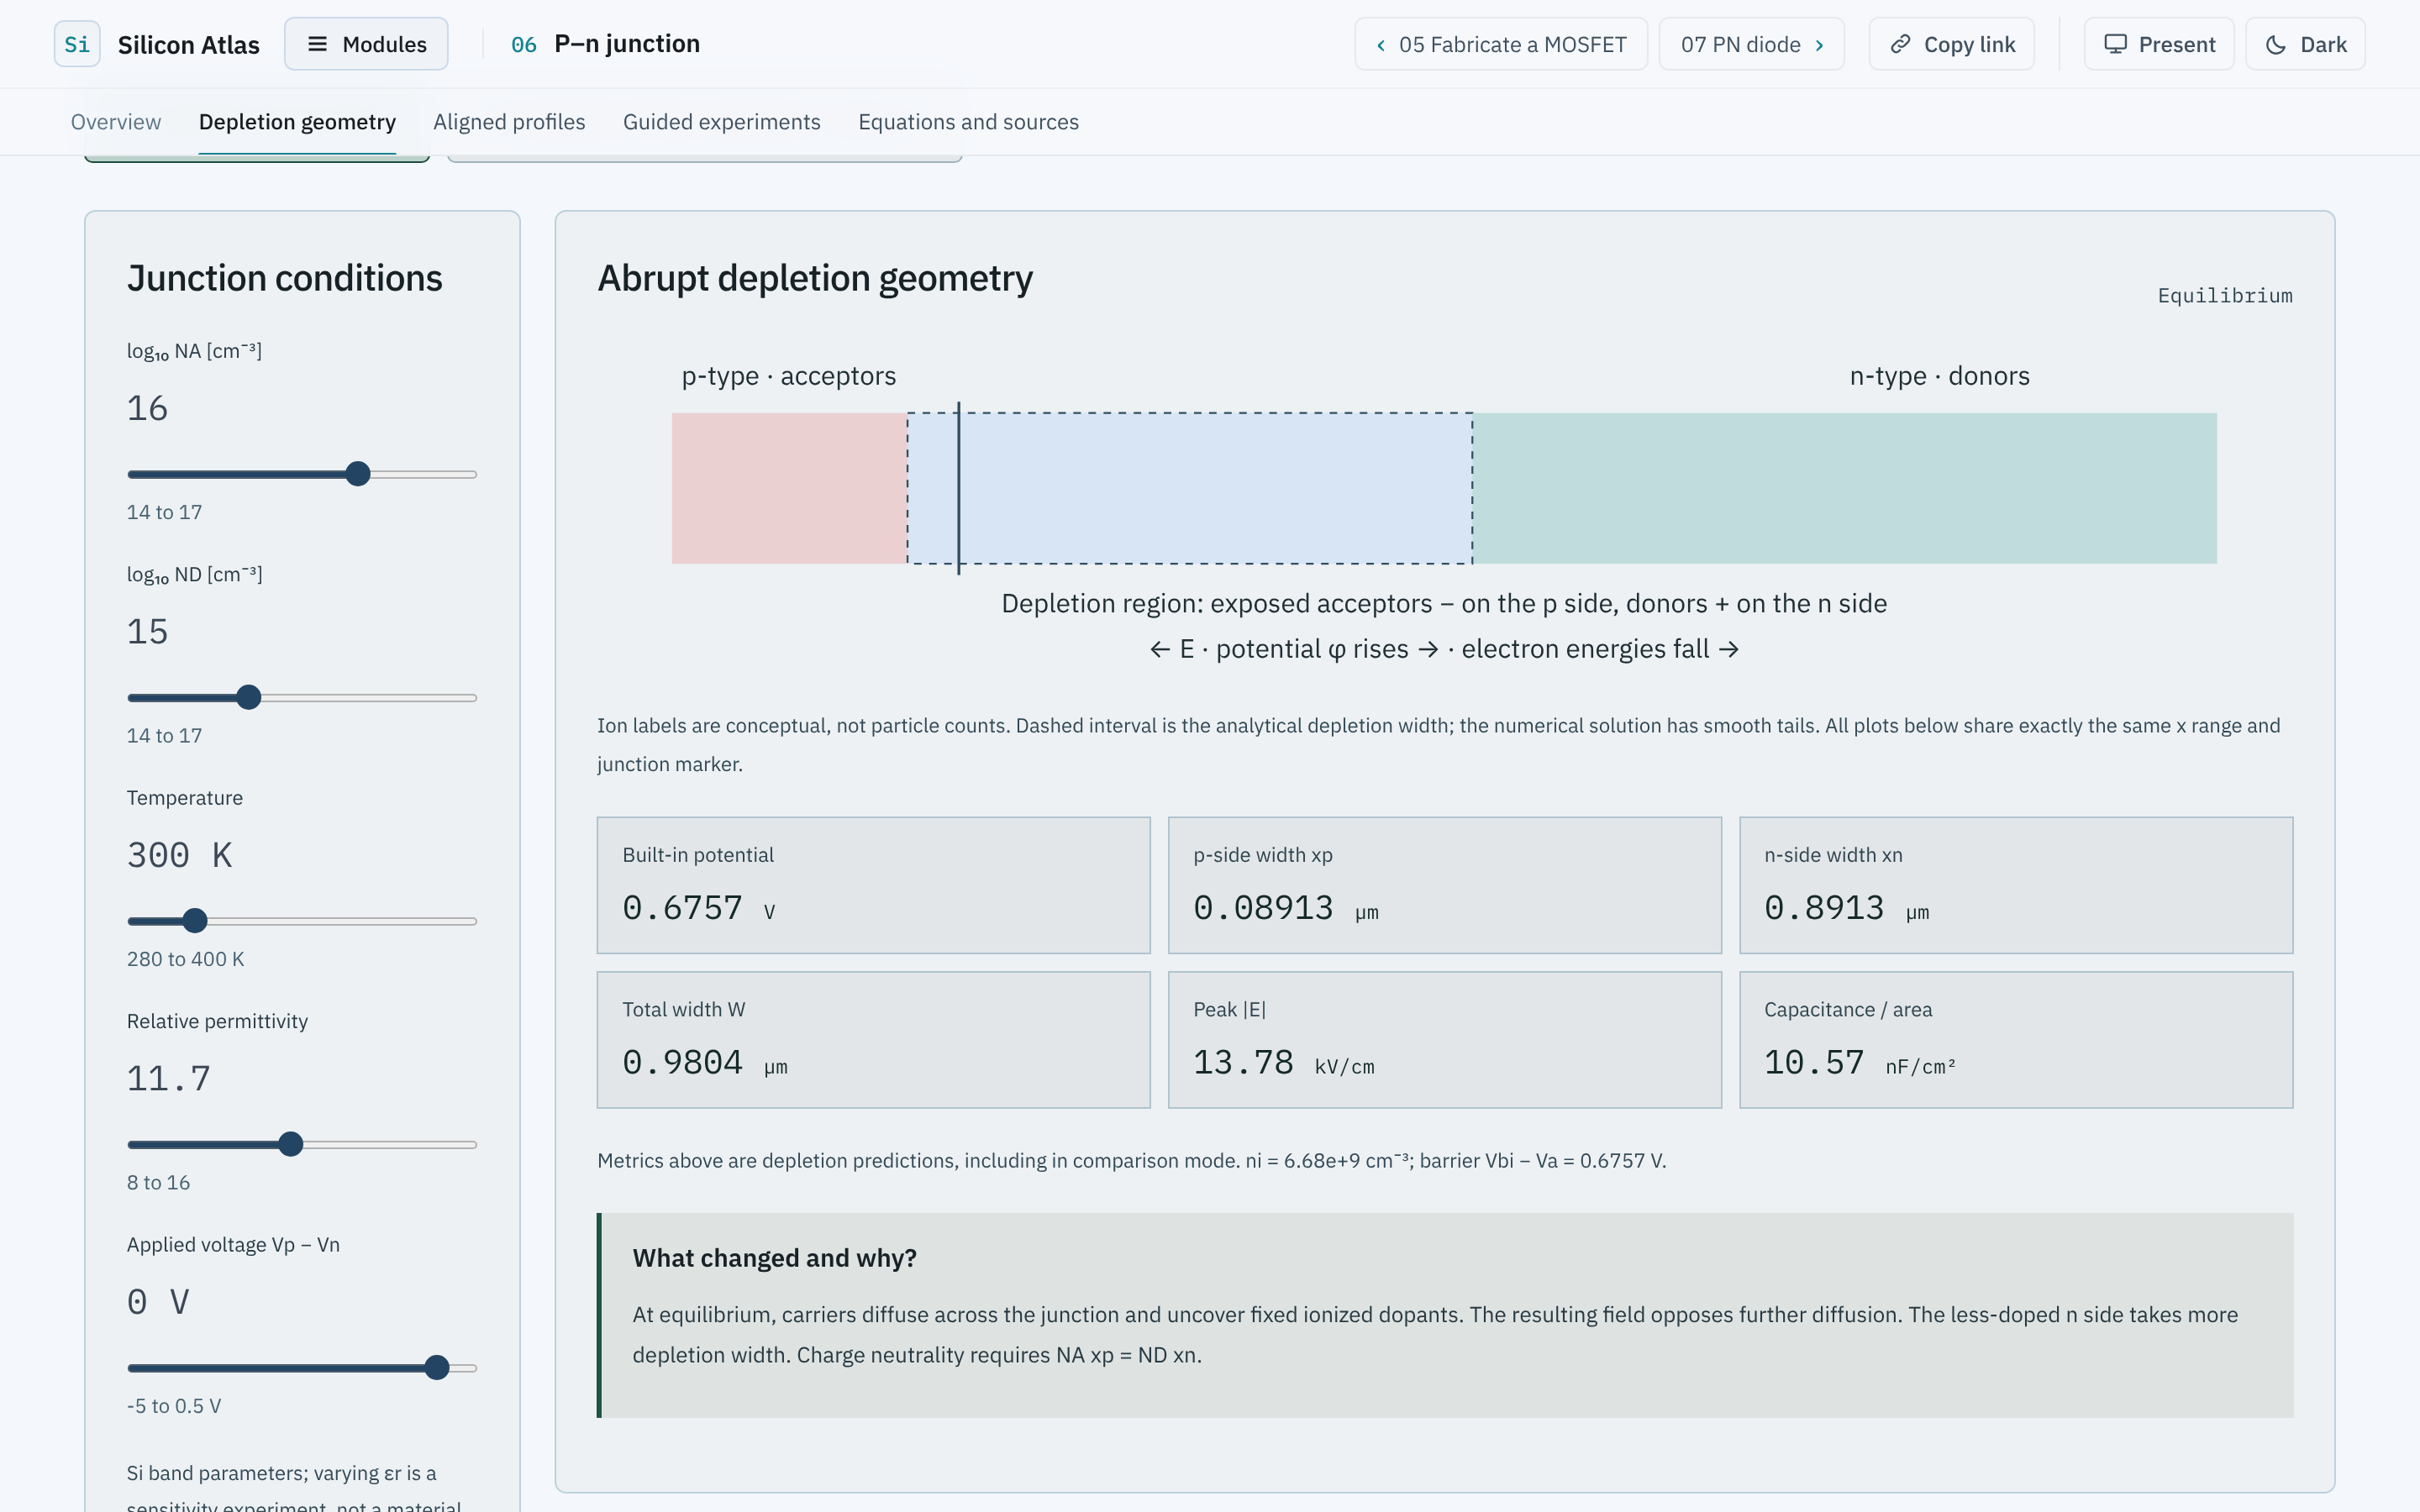
\includegraphics[width=0.92\textwidth]{fig_ui.png}
\caption{The p--n junction lab in a browser (light theme). Top: the shared app bar with the modules menu, previous and next lab, and section shortcuts. Left: junction controls. Right: the depletion geometry, the computed metrics for the default $N_A=10^{16}$~cm$^{-3}$, $N_D=10^{15}$~cm$^{-3}$ junction at 300~K, and the ``What changed and why?'' panel. The aligned field, potential, and band plots follow below.}
\label{fig:ui}
\end{figure*}

%======================================================================
\section{Software Architecture}\label{sec:arch}
%======================================================================
Fig.~\ref{fig:arch} shows how the platform is organized. The physics lives in eleven TypeScript kernels (about 3{,}200 lines) that do not import any interface code. Every kernel works in SI units internally, converts units only at the interface, validates its inputs, and throws a descriptive error when an input is outside its supported range. The interface (about 13{,}000 lines of React and SVG) calls the kernels and plots their output with Recharts. Each lab is loaded on demand, so the first page load transfers about 260~kB of application code plus the lab in view.

All kernels read silicon, GaAs, and SiO$_2$ parameters from one module that holds the values of Neamen's Appendix~B \cite{neamen2012} and the exact SI constants \cite{codata2018}. A test enforces that every kernel derives the same intrinsic density and effective densities of states. An earlier version had duplicated these constants across six kernels, and two of them disagreed with the textbook tables (Section~\ref{sec:params}). Lab settings that differ from their defaults are mirrored into the URL, so a link restores a setup exactly, and a failure caused by an impossible linked value shows a message rather than a blank page.

The 89 automated test groups use Node's built-in test runner. They check analytical limits, conservation laws, independent quadratures, and grid and time-step refinement for each kernel. A continuous-integration workflow runs them, the formatter, and the production build on every change, and a second workflow publishes the site.

\begin{figure}[t]
\centering
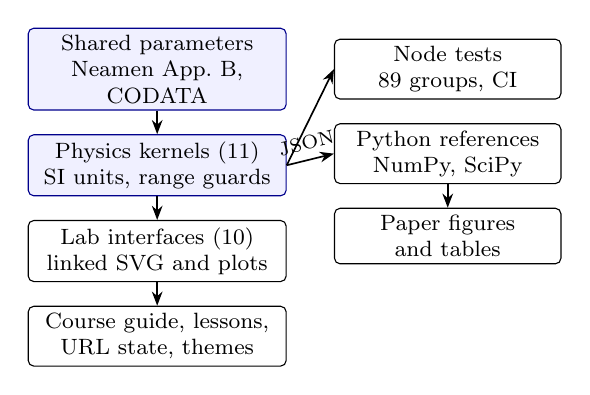
\begin{tikzpicture}[font=\footnotesize, node distance=3mm,
  box/.style={draw, rounded corners=2pt, align=center, minimum height=6.5mm, inner sep=2.5pt, fill=white, text width=#1},
  box/.default=30mm,
  core/.style={box=#1, fill=blue!6, draw=blue!55!black},
  core/.default=30mm,
  arr/.style={-{Stealth[length=1.8mm]}, semithick}]
\node[core=31mm] (mat) {Shared parameters\\Neamen App.~B, CODATA};
\node[core=31mm, below=of mat] (ker) {Physics kernels (11)\\SI units, range guards};
\node[box=31mm, below=of ker] (ui) {Lab interfaces (10)\\linked SVG and plots};
\node[box=31mm, below=of ui] (shell) {Course guide, lessons,\\URL state, themes};
\node[box=27mm, right=6mm of mat] (tests) {Node tests\\89 groups, CI};
\node[box=27mm, below=of tests] (py) {Python references\\NumPy, SciPy};
\node[box=27mm, below=of py] (fig) {Paper figures\\and tables};
\draw[arr] (mat) -- (ker); \draw[arr] (ker) -- (ui); \draw[arr] (ui) -- (shell);
\draw[arr] (ker.east) -- (tests.west);
\draw[arr] (ker.east) -- node[above, font=\scriptsize, sloped]{JSON} (py.west);
\draw[arr] (py) -- (fig);
\end{tikzpicture}
\caption{Organization of Silicon Atlas. The same kernels serve the browser, the automated tests, and the data behind this paper's figures, which an independent Python script checks.}
\label{fig:arch}
\end{figure}

%======================================================================
\section{Physical Models and Numerical Methods}\label{sec:models}
%======================================================================
This section states each model as implemented. Symbols follow \cite{neamen2012}; temperatures are in kelvin and all quantities are in SI units unless noted.

\subsection{Shared parameters and intrinsic density}\label{sec:params}
Silicon uses $E_g=1.12$~eV, $\chi=4.01$~eV, $\varepsilon_r=11.7$, $N_c=2.8\times10^{19}$ and $N_v=1.04\times10^{19}$~cm$^{-3}$ at 300~K scaled as $(T/300)^{3/2}$, and lattice mobilities of 1350 and 480~cm$^2$/V\,s \cite{neamen2012}. The band gap and mobilities are held at their 300~K values. The intrinsic density is computed from the same parameters,
\begin{equation}
n_i=\sqrt{N_cN_v}\,\exp\!\left(-E_g/2kT\right),
\end{equation}
which gives $6.68\times10^9$~cm$^{-3}$ at 300~K. This differs from the $1.5\times10^{10}$~cm$^{-3}$ used in the textbook's worked examples and from the value near $9.65\times10^9$~cm$^{-3}$ reported in the device literature \cite{sproul1991,altermatt2003}. We keep the self-consistent value so that $n_0p_0=n_i^2$ holds exactly with the parameters used for the band diagrams, and the labs state the discrepancy where it matters. Two inconsistencies were removed in the process: the MOS lab had used $\chi=4.05$~eV, common in other texts \cite{sze2007}, and the photonics lab had used $E_g=1.424$~eV for GaAs instead of the tabulated 1.42~eV.

\subsection{Materials and quantum foundations}
\emph{Segregation.} During Czochralski growth with complete mixing in the melt and no diffusion in the solid, the solid concentration at fraction solidified $f$ is \cite{scheil1942}
\begin{equation}
C_s(f)=kC_0(1-f)^{k-1},
\end{equation}
and the lab computes the exact average over any retained interval $[a,b]$ from the integral $C_0[(1-a)^k-(1-b)^k]/(b-a)$ (Fig.~\ref{fig:scheil}).

\begin{figure}[t]
\centering
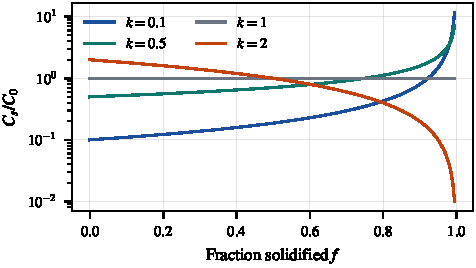
\includegraphics[width=\columnwidth]{fig_scheil.pdf}
\caption{Scheil profiles along a Czochralski crystal for four segregation coefficients. Impurities with $k<1$ are rejected into the melt and pile up in the last part of the crystal to solidify. The lab plots the same curves and checks interval averages against the exact integral.}
\label{fig:scheil}
\end{figure} The growth lab uses a lumped heat balance at the interface, $Q_{\text{out}}=hA(T_b-T_m)+\rho A v_pL_f$, to show how melt temperature and pull speed set the crystal diameter under a fixed cooling rate.

\emph{Wells, barriers, and bands.} The infinite well has $E_n=n^2\pi^2\hbar^2/2mL^2$. Transmission through a rectangular barrier of height $U_0$ and width $d$ uses the exact closed form \cite{neamen2012}, written with $\sinh(z)/z$ so that it stays finite at $E=U_0$. Band formation is illustrated with a one-orbital, nearest-neighbor chain, $E(k)=-2t\cos ka$, whose curvature gives the effective mass $m^*=\hbar^2/(d^2E/dk^2)$ and whose negative band-top mass motivates the hole \cite{ashcroft1976}. The chain is labeled as an illustration, not a silicon band structure.

\subsection{Equilibrium carriers}
For a uniform sample with donors $N_D$ and acceptors $N_A$, the lab solves charge neutrality
\begin{equation}
p+N_D^+-n-N_A^-=0
\end{equation}
for the Fermi level by bracketed bisection, with incomplete ionization (degeneracy factors 2 and 4) and either Boltzmann statistics or the Fermi--Dirac integral
\begin{equation}
n=N_c\,\tfrac{2}{\sqrt\pi}F_{1/2}(\eta),\quad F_{1/2}(\eta)=\int_0^\infty\frac{\epsilon^{1/2}\,d\epsilon}{1+e^{\epsilon-\eta}}.
\end{equation}
The substitution $\epsilon=u^2$ removes the endpoint singularity, and composite Simpson quadrature with 128 panels is used. In Boltzmann mode the lab flags results within $3kT$ of a band edge as outside the nondegenerate range.

\subsection{Transport}
The transport lab evolves the excess minority-carrier density $u(x,t)$ on a bar under a uniform field,
\begin{equation}
\frac{\partial u}{\partial t}=-\frac{\partial}{\partial x}\left(v u - D\frac{\partial u}{\partial x}\right)+G-\frac{u}{\tau},
\end{equation}
with $v=\mp\mu E$ for electrons and holes. A conservative cell-centered finite-volume method uses upwind drift fluxes, centered diffusion fluxes, and explicit Euler steps limited by a stability bound \cite{leveque2002}. Absorbing, reflecting, and periodic boundaries are available, and a ledger tracks generation, recombination, and boundary transfer so that particle conservation is visible. The Einstein relation $D=\mu kT/q$ can link the two coefficients. Low injection is flagged above 1\% of the majority density.

\subsection{Fabrication}
The process lab follows the course's four-mask metal-gate nMOS flow in 26 steps. Oxide growth uses the Deal--Grove model \cite{dealgrove1965},
\begin{equation}
x^2+Ax=B(t+\tau),
\end{equation}
with coefficients for wet and dry oxidation and a (100) correction; the thin dry-oxide regime where the model underestimates growth \cite{massoud1985} is flagged. Phosphorus diffusion with constant diffusivity gives either a constant-source profile $C_s\,\mathrm{erfc}(z/2\sqrt{Dt})$ or a limited-dose Gaussian $(Q/\sqrt{\pi Dt})e^{-z^2/4Dt}$, with $\mathrm{erfc}$ evaluated by the Abramowitz--Stegun rational approximation 7.1.26 \cite{abramowitz1964}. The junction depth is found by bisection. Lithography convolves rectangular clear areas with a Gaussian and applies a positive-resist threshold, and etching acts on a $160\times80$ height field. Connected-component checks identify source, gate, and drain contacts and detect faults. The finished device can be reduced to an oxide thickness, channel length and width, and substrate doping and imported into the MOS lab; the nominal recipe gives $t_{ox}=54.8$~nm, $L=10.5$~\si{\micro\metre}, and $W=8.5$~\si{\micro\metre}.

\subsection{P--n junction}
In the depletion approximation for an abrupt junction,
\begin{gather}
V_{bi}=\frac{kT}{q}\ln\frac{N_AN_D}{n_i^2},\\
W=\sqrt{\frac{2\varepsilon_s(V_{bi}-V_a)}{q}\left(\frac{1}{N_A}+\frac{1}{N_D}\right)},\\
|E_{\max}|=\frac{2(V_{bi}-V_a)}{W},\qquad C'=\frac{\varepsilon_s}{W},
\end{gather}
and the field and potential are piecewise linear and quadratic \cite{neamen2012}. At zero bias the lab also solves the full Poisson--Boltzmann equation,
\begin{equation}
\frac{d^2\phi}{dx^2}=-\frac{q}{\varepsilon_s}\Big(n_ie^{-\phi/V_T}-n_ie^{\phi/V_T}+N_D(x)-N_A(x)\Big),
\end{equation}
with $\phi$ referenced to the intrinsic level. It uses a cell-centered finite-volume grid with the doping step on a cell face, Dirichlet values from the neutral reservoirs, and Newton iteration with an exact tridiagonal Jacobian and backtracking. The lab reports the iteration count and residual, compares the net charge with the field at the domain boundaries, and recomputes the solution on a doubled grid and a padded domain so that discretization error is visible. Results are withheld below a barrier of $6kT/q$, above 1\% injection, or above a field of 100~kV/cm, which is a conservative teaching limit and not a breakdown model.

\subsection{Diode}
The diode lab uses the Shockley model with finite neutral regions \cite{shockley1949},
\begin{gather}
I=I_s\!\left(e^{V/V_T}-1\right),\\
I_s=qAn_i^2\!\left[\frac{D_n}{L_nN_A}\coth\frac{W_p}{L_n}+\frac{D_p}{L_pN_D}\coth\frac{W_n}{L_p}\right],
\end{gather}
which approaches both the long- and short-diode limits. Optional series resistance is solved by a bracketed root, and an optional depletion-region recombination term with ideality factor 2 \cite{sah1957} is labeled as empirical. Switching uses charge control, $dQ/dt=I-Q/\tau_Q$, with $\tau_Q$ taken from the steady stored charge.

\subsection{MOS capacitor and MOSFET}
For a p-type substrate with majority and minority densities $p_0$ and $n_0$, the semiconductor charge follows from the first integral of Poisson's equation \cite{neamen2012},
\begin{equation}
Q_s=-\operatorname{sgn}(\psi_s)\frac{\sqrt2\,\varepsilon_sV_T}{L_D}F(\psi_s),\quad L_D=\sqrt{\frac{\varepsilon_sV_T}{qp_0}},
\end{equation}
with $F^2=(e^{-u}+u-1)+(n_0/p_0)(e^{u}-u-1)$ and $u=\psi_s/V_T$. The gate voltage is $V_G=V_{FB}+\psi_s-Q_s/C_{ox}$, which the lab inverts for $\psi_s$, and the quasi-static capacitance is $-dQ_s/dV_G$. A high-frequency curve is shown separately as an approximation that holds the inversion charge fixed and is omitted near flat band. The transistor uses the long-channel square-law model with a source-referenced body effect \cite{pao1966,brews1978},
\begin{equation}
I_D=\beta\Big[(V_{GS}-V_T)V_{DS}-\tfrac12V_{DS}^2\Big],\quad \beta=\mu C_{ox}\frac{W}{L},
\end{equation}
which saturates at $V_{DS}=V_{GS}-V_T$; channel-length modulation is an optional empirical factor.

\subsection{Photonic devices}
Photon energy and flux follow from the wavelength. Generation follows Beer--Lambert absorption, $G(z)=\alpha\Phi e^{-\alpha z}$, and the photocurrent is $I_{ph}=q\Phi A\eta$ with an assumed collection efficiency. The solar cell is an illuminated ideal diode with optional series and shunt resistance; the lab finds $V_{oc}$, $I_{sc}$, and the maximum-power point and accounts for all incident power. The absorption coefficients are illustrative curves for indirect and direct gaps and are labeled as such; replacing them with tabulated silicon data \cite{green2008} is future work.

\subsection{Measurement bench}
The bench reproduces course measurements with square-law transistors and lumped capacitances. Resistor stations separate sheet resistance from contact resistance by regression over length. Transistor stations extract threshold voltage and mobility from linear and saturation sweeps. Inverter, loaded-transient, and five-stage ring-oscillator stations solve Kirchhoff's current law at each node and integrate the node capacitances with fourth-order Runge--Kutta steps. No oscillation frequency is assumed: the ring starts from its solved equilibrium plus a small perturbation, and the frequency emerges from the simulation. Optional seeded noise, quantization, contact resistance, and oscilloscope loading show how instruments change a measurement.

%======================================================================
\section{Verification}\label{sec:verification}
%======================================================================
\subsection{Method}
A script runs the same TypeScript kernels used in the browser and writes their outputs to JSON. A separate Python script recomputes every reference result with NumPy and SciPy from the textbook formulas, with no shared code, and reports the largest error. For closed-form models this checks the implementation, not the model: a kernel and its reference that evaluate the same formula should agree to rounding error, and they do. Where an independent method exists, the reference uses it, for example a transfer-matrix solution for barrier transmission, adaptive quadrature for the Fermi--Dirac integral, and an independent neutrality solve for the carrier densities. For numerical schemes the script measures convergence under refinement. Table~\ref{tab:verify} summarizes the results.

\begin{table}[t]
\centering
\caption{Verification summary. Errors are the largest relative errors over each sweep unless noted. Numerical schemes report observed convergence.}
\label{tab:verify}
\scriptsize
\setlength{\tabcolsep}{3pt}
\begin{tabular}{@{}l l l@{}}
\toprule
Check & Reference & Max. error \\
\midrule
Scheil profile and interval averages & Closed form & $3.8\times10^{-15}$ \\
Infinite-well levels & Closed form & $1.6\times10^{-16}$ \\
Barrier transmission & Transfer matrix & $1.0\times10^{-15}$ abs. \\
$F_{1/2}(\eta)$, 128 panels & Adaptive quadrature & $1.1\times10^{-8}$ \\
$n(T)$, 40--800~K, $N_D=10^{15}$ & Independent solve & $1.8\times10^{-10}$ \\
Diffusion variance $\sigma_0^2+2Dt$ & Analytic & $7.8\times10^{-12}$ \\
Drift centroid $x_0-\mu Et$ & Analytic & $1.4\times10^{-19}$~m \\
Recombination decay $e^{-t/\tau}$ & Analytic & $8.0\times10^{-3}$ \\
Deal--Grove thickness & Closed form & $3.4\times10^{-15}$ \\
Gaussian dose conservation & Quadrature & $2.3\times10^{-16}$ \\
erfc profile (A--S 7.1.26) & SciPy erfc & $1.4\times10^{-3}$ \\
Depletion $V_{bi}$, $W$, $E_{\max}$, $W(V_R)$ & Closed form & $<10^{-15}$ \\
Neamen Ex.\ 7.1--7.5 ($n_i=1.5\times10^{10}$) & Textbook & $3.7\times10^{-3}$ \\
Poisson--Boltzmann charge balance & Boundary field & $7.9\times10^{-16}$ \\
Poisson--Boltzmann peak field & Richardson & order 0.92--0.98 \\
Diode $I(V)$, area $A$ and $2A$ & Shockley (SciPy) & $3.4\times10^{-16}$ \\
MOS quasi-static $C$--$V$ & Independent $Q_s(\psi_s)$ & $6.6\times10^{-6}\,C_{ox}$ \\
MOSFET output curves & Square law & $1.7\times10^{-16}$ \\
Solar $V_{oc}$, $I_{sc}$, $P_{\max}$ & Closed form, optimizer & $1.7\times10^{-16}$ \\
Ring frequency, time step halved & Self-convergence & $6.1\times10^{-6}$ \\
Bench extraction, ideal instruments & Model inputs & $2.2\times10^{-16}$ \\
\bottomrule
\end{tabular}
\end{table}

\subsection{Materials, carriers, and transport}
Barrier transmission agrees with the transfer-matrix solution to $10^{-15}$ across energies below and above the barrier and across five orders of magnitude of tunneling probability. The Fermi--Dirac integral agrees with adaptive quadrature to $1.1\times10^{-8}$ for $-10\le\eta\le20$; the error is largest deep in the degenerate range (Fig.~\ref{fig:eq}, right) and falls to $5\times10^{-9}$ with 512 panels. The electron density of an $N_D=10^{15}$~cm$^{-3}$ sample agrees with an independent solve from 40 to 800~K, through freeze-out, the extrinsic plateau, and the intrinsic range (Fig.~\ref{fig:eq}, left). At this doping the Boltzmann and Fermi--Dirac results are indistinguishable, as expected for a nondegenerate sample.

\begin{figure*}[t]
\centering
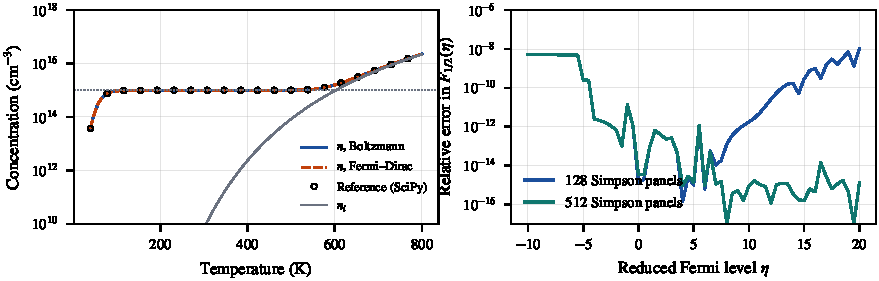
\includegraphics[width=0.49\textwidth]{fig_equilibrium.pdf}\hfill
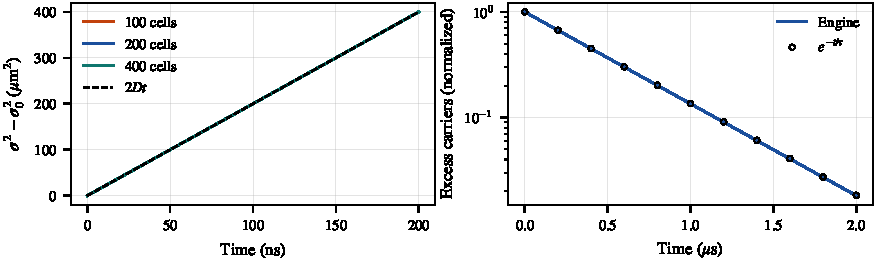
\includegraphics[width=0.49\textwidth]{fig_transport.pdf}
\caption{Left pair: electron density versus temperature for $N_D=10^{15}$~cm$^{-3}$ in silicon (freeze-out, extrinsic, and intrinsic regimes) against an independent SciPy solve, and the relative error of the Fermi--Dirac integral. Right pair: growth of a diffusing packet's variance on three grids against $2Dt$, and decay of a uniform excess against $e^{-t/\tau}$.}
\label{fig:eq}
\end{figure*}

The finite-volume transport solver conserves particles exactly with reflecting boundaries, and the variance of a diffusing Gaussian follows $\sigma_0^2+2Dt$ to $10^{-11}$ on all three grids (Fig.~\ref{fig:eq}). Pure drift moves the centroid by exactly $\mu Et$. The upwind scheme adds numerical diffusion to a drifting packet, and that artificial spreading falls at an observed order of 1.1 as the grid is refined, consistent with a first-order upwind method \cite{leveque2002}. The recombination decay differs from $e^{-t/\tau}$ by up to 0.8\% because of the explicit time step; the test suite confirms that this error falls as the step is reduced.

\subsection{Fabrication}
Oxide thickness agrees with the closed-form Deal--Grove solution to rounding error at wet and dry conditions, and growing for 1~h twice equals growing for 2~h once. Fig.~\ref{fig:fab} shows the transition from the linear limit $(B/A)t$ to the parabolic limit $\sqrt{Bt}$. The Gaussian profile conserves its dose to $10^{-16}$. The constant-source profile differs from SciPy's $\mathrm{erfc}$ by up to $1.4\times10^{-3}$ in relative terms, deep in the tail where the Abramowitz--Stegun approximation's absolute error of $1.5\times10^{-7}$ becomes a relative one; the junction depth is unaffected at the doping levels used.

\begin{figure*}[t]
\centering
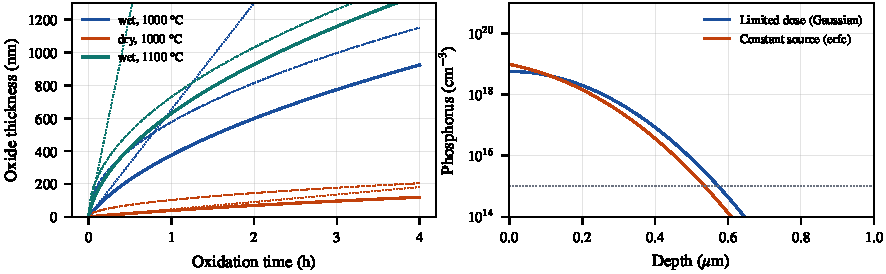
\includegraphics[width=0.49\textwidth]{fig_fabrication.pdf}\hfill
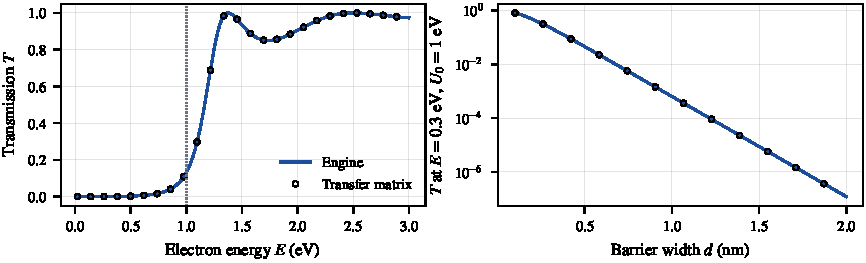
\includegraphics[width=0.49\textwidth]{fig_quantum.pdf}
\caption{Left pair: oxide thickness for three oxidation conditions with the linear (dotted) and parabolic (dashed) limits, and phosphorus profiles for limited-dose and constant-source diffusion; the dotted line is the substrate doping. Right pair: transmission through a 1~eV, 1~nm barrier against a transfer-matrix solution, and its exponential decrease with barrier width at 0.3~eV.}
\label{fig:fab}
\end{figure*}

\subsection{Junction}
The depletion results reproduce their closed forms exactly, and the earlier junction kernel, which uses the textbook's $n_i=1.5\times10^{10}$~cm$^{-3}$, reproduces Neamen's Examples 7.1--7.5 to within 0.37\%, the rounding of the printed answers. For the default junction ($N_A=10^{16}$, $N_D=10^{15}$~cm$^{-3}$) the lab gives $V_{bi}=0.676$~V and $W=0.980$~\si{\micro\metre}.

The Poisson--Boltzmann solver converges in four Newton iterations on every grid from 40 to 1280 cells per side, and its net charge matches the boundary field to $8\times10^{-16}$. Its peak field converges at first order, with observed orders of 0.92 to 0.98 (Fig.~\ref{fig:jn}, right). The order is first rather than second because the abrupt doping step makes the solution's curvature discontinuous at the junction, and the displayed cell field averages two face values there. At 320 cells per side the remaining error in the peak field is below 0.5\%, small compared with the 3.1\% physical difference between the full solution and the depletion approximation, whose peak is higher because it ignores the mobile carriers in the depletion tails (Fig.~\ref{fig:jn}, left). The lab shows this difference as a teaching point.

\begin{figure*}[t]
\centering
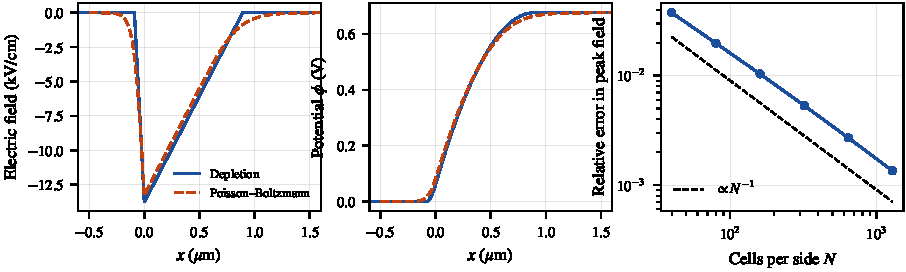
\includegraphics[width=\textwidth]{fig_junction.pdf}
\caption{Default junction ($N_A=10^{16}$, $N_D=10^{15}$~cm$^{-3}$, 300~K). Left and center: electric field and potential from the depletion approximation and the Poisson--Boltzmann solver. Right: relative error in the solver's peak field against a Richardson-extrapolated reference, showing first-order convergence.}
\label{fig:jn}
\end{figure*}

\subsection{Devices and measurements}
Diode currents at areas $A$ and $2A$ agree with an independent Shockley calculation to rounding error, and the semilog slope is 59.53~mV per decade, equal to $V_T\ln10$ at 300~K (Fig.~\ref{fig:dev}). The quasi-static MOS capacitance agrees with an independent reference, which inverts $V_G(\psi_s)$ on a fine grid and differentiates numerically, to within $6.6\times10^{-6}C_{ox}$, and the surface potential to $3\times10^{-7}$~V (Fig.~\ref{fig:mos}). The flat-band voltage and threshold for the default nMOS gate are $-0.350$~V and $0.814$~V. Transistor output curves match the square law exactly and are continuous at pinch-off.

\begin{figure*}[t]
\centering
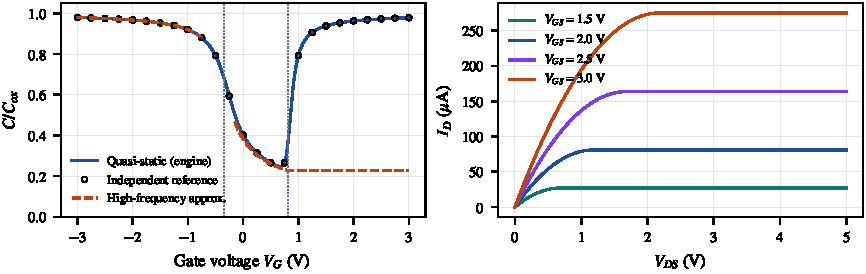
\includegraphics[width=0.72\textwidth]{fig_mos.pdf}
\caption{Left: quasi-static C--V of the default nMOS capacitor against an independent reference, and the high-frequency approximation; dotted lines mark flat band and threshold. Right: long-channel output characteristics.}
\label{fig:mos}
\end{figure*}

\begin{figure*}[t]
\centering
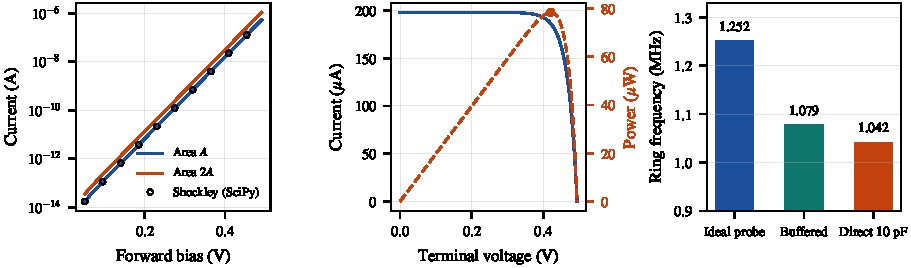
\includegraphics[width=\textwidth]{fig_devices.pdf}
\caption{Left: diode current for areas $A$ and $2A$ against the Shockley equation. Center: solar-cell current and power under monochromatic illumination, with the maximum-power point. Right: five-stage ring-oscillator frequency with an ideal probe, a buffered probe, and a 10~pF probe connected directly.}
\label{fig:dev}
\end{figure*}

The solar-cell open-circuit voltage, short-circuit current, and maximum power agree with closed forms and a bounded optimizer, giving a fill factor of 0.80 under the default illumination, and the incident power is accounted for to $10^{-20}$~W. The ring oscillator's frequency changes by $6\times10^{-6}$ when the time step is halved, and its period agrees with ten measured stage delays to $8\times10^{-6}$. With the default stage parameters it oscillates at 1.252~MHz. A buffered probe lowers this to 1.079~MHz and a directly connected 10~pF probe to 1.042~MHz, which is the loading effect students observe on the real bench (Fig.~\ref{fig:dev}, right). With noise, quantization, and contact resistance turned off, the bench's extraction routines recover the parameters the model was given: a sheet resistance of 0.2~$\Omega/\square$ from the length regression, and a threshold of 2~V and mobility of 500~cm$^2$/V\,s from the linear-region fit, each to rounding error. This round trip confirms that any spread students see once the instrument models are turned on comes from those models and not from the extraction code.

%======================================================================
\section{A Connected Activity}
%======================================================================
The labs are designed so that a single activity can cross several of them. In one sequence a student runs the nMOS process in module 05 at its tested settings, inspects the finished device in cross-section, and loads a contact-misalignment fault to see which terminal fails and why. The student then imports the nominal device into module 08, which reduces it to $t_{ox}=54.8$~nm, $L=10.5$~\si{\micro\metre}, $W=8.5$~\si{\micro\metre}, and $N_A=10^{15}$~cm$^{-3}$, sweeps the gate through accumulation, depletion, and inversion, and reads the threshold and output characteristics. Finally, in module 10, the student extracts threshold and mobility from simulated sweeps by two methods and sees how sweep spacing and instrument noise change the extracted values. Each step states what it inherited from the previous one, and every number can be traced to an equation in the lab's panel.

%======================================================================
\section{Limitations}\label{sec:limits}
%======================================================================
The models are deliberately simple, and their limits are stated in each lab.
\begin{itemize}
\item \emph{Verification, not validation.} All checks are against theory or independent calculation. No result has been compared with measured data, and agreement with the textbook model does not show that the model describes a real device beyond its stated range.
\item \emph{Material parameters.} The band gap and mobilities are held at their 300~K values, so the equilibrium lab's high-temperature behavior and high-doping conductivities are qualitative. A Varshni band gap \cite{varshni1967} and a Caughey--Thomas mobility \cite{caughey1967} are natural, still-simple extensions. The intrinsic density is internally consistent but differs from both the textbook's example value and the literature value (Section~\ref{sec:params}).
\item \emph{Devices.} The Poisson--Boltzmann solver is equilibrium only; there is no biased drift--diffusion solution, no high injection, and no breakdown. The MOSFET is long-channel, without subthreshold conduction or short-channel effects. Recombination in the depletion region is empirical rather than a spatial Shockley--Read--Hall solution \cite{shockleyread1952,hall1952}.
\item \emph{Optics and process.} Absorption coefficients are illustrative. The process flow is one-dimensional in its diffusion model, ignores concentration-dependent and lateral diffusion, and does not model resist chemistry.
\item \emph{Education.} The learning goals, guided experiments, and self-check questions were written for the course, but no study of their effect on learning has been carried out.
\end{itemize}

%======================================================================
\section{Conclusion}
%======================================================================
Silicon Atlas shows that the models of an introductory semiconductor devices course can be built into one set of connected, browser-based labs that a student can explore and an instructor can audit. Every kernel draws on one parameter set, refuses inputs outside its range, and agrees with independently computed references, to rounding error for closed forms and at the expected order for the numerical schemes. The next steps are to replace the illustrative and fixed parameters noted above with cited data, to compare selected results with laboratory measurements, and to gather feedback from instructors and students on accuracy, fit to the course, and usability. The source code, tests, and the scripts that generate every figure and table in this paper are released under the MIT license at \url{\repourl}, and the labs run at \url{\demourl}.

\bibliographystyle{IEEEtran}
\bibliography{refs}

\end{document}
